\documentclass[journal]{IEEEtran}
\usepackage{amsmath,amssymb,amsfonts}
\usepackage{graphicx}
\usepackage{booktabs}
\usepackage{url}
\usepackage{xcolor}
\usepackage[hidelinks]{hyperref}
\usepackage{cite}
\usepackage[noend]{algpseudocode}
\usepackage{algorithm}

\begin{document}

\title{Explainable Meta-Learning with Graph Intelligence for\\
Cognitive UAV Swarms in Electronic-Warfare Environments}

\author{Adeel~Ahmad
\thanks{The author is with the Department of Electrical/Computer Engineering.
Code and data: \url{https://github.com/adeliusa486/XM-MADRL-eXplainable-Meta-learning-Multi-Agent-DRL}.}}

\markboth{Preprint, August 2026}{Ahmad: Explainable Meta-Learning for Cognitive UAV Swarms}
\maketitle

\begin{abstract}
Cognitive unmanned aerial vehicle (UAV) swarms operating in electronic-warfare
(EW) environments must navigate GPS-denied airspace, share a congested radio
spectrum under adaptive jamming, coordinate as a team, and remain interpretable
for mission-critical use. Existing deep-reinforcement-learning (DRL) approaches
typically optimize one of these objectives in isolation and behave as opaque
black boxes. We present \emph{XM-MADRL}, a unified framework that integrates
multi-modal transformer-based sensing, graph-neural-network (GNN) swarm
communication, multi-agent proximal policy optimization (MAPPO), model-agnostic
meta-learning (MAML) for rapid task adaptation, and SHAP-based explainability. A
key architectural insight, validated by ablation, is that swarm-level graph
aggregation \emph{over-smooths} the local spectrum-sensing signal each agent
needs for channel selection; we therefore \emph{decouple} the policy into a
coordinated navigation head and a local spectrum head. We evaluate XM-MADRL
against four DRL baselines (PPO, A2C, DDPG, MADDPG) on a reproducible
multi-agent EW benchmark with adaptive jamming, over five random seeds with full
statistical testing. XM-MADRL attains the highest mission-success rate
among collision-free methods together with zero collisions, while remaining
competitive on communication reliability and anti-jamming; the decoupled spectrum
head more than doubles packet-delivery ratio over a naive graph-only policy, and
a constellation-based classifier attains $84\%$ modulation-recognition accuracy.
We report results honestly, including a modest energy premium and a residual
anti-jamming gap relative to strong single-objective baselines.
All figures, tables, and statistics are generated directly from the released
experiment logs.
\end{abstract}

\begin{IEEEkeywords}
Cognitive UAV networks, multi-agent reinforcement learning, meta-learning,
explainable AI, graph neural networks, electronic warfare, spectrum access.
\end{IEEEkeywords}

\section{Introduction}
\IEEEPARstart{U}{nmanned} aerial vehicles (UAVs) have become a transformative
technology for surveillance, reconnaissance, spectrum monitoring, and electronic
warfare (EW)~\cite{choi2023modular,xu2023pursuing}. Cognitive UAV networks are
expected to sense their environment, learn from experience, and autonomously
adapt in dynamic, adversarial, spectrum-congested conditions~\cite{jiang2022multiagent}.
Deep reinforcement learning (DRL) has emerged as a powerful tool for such
autonomy, achieving strong results in navigation~\cite{choi2023modular,xu2023multiuav},
dynamic spectrum access~\cite{dong2022dynamic,wang2022usage}, and
anti-jamming~\cite{zheng2022airborne,chen2022distributed}.

Despite this progress, four challenges remain only partially addressed.
\emph{Scalability and coordination:} many DRL controllers degrade as the swarm
grows and inter-agent communication becomes essential~\cite{liu2023task}.
\emph{Adaptability:} policies trained in one setting transfer poorly to unseen
jamming patterns and mission conditions, and expensive retraining is
required~\cite{hieu2022transferable}. \emph{Robustness under adaptive jamming:}
many anti-jamming methods assume simplified, static adversaries~\cite{chen2022distributed}.
\emph{Interpretability:} DRL policies are opaque, which undermines trust in
mission-critical operations~\cite{lundberg2017unified}. Crucially, these are
usually studied in isolation, whereas a deployable cognitive UAV swarm must
satisfy them \emph{jointly}.

Addressing these challenges jointly is non-trivial because the underlying
objectives interact and even conflict: aggressive spectrum exploration improves
throughput but drains energy; tight formation aids coordination but raises
collision risk; and larger, more expressive models improve capacity but are
harder to train and to interpret. A practical framework must therefore expose
these trade-offs explicitly rather than optimize a single proxy. A further,
subtler difficulty---which we identify and resolve in this work---is that the
very mechanism used for swarm coordination (graph message passing) can degrade a
capability it is not meant to touch: local spectrum sensing. We show that naive
graph aggregation \emph{over-smooths} the per-agent radio-frequency (RF) features
required for channel selection, and that a decoupled policy resolves this.

\textbf{Contributions.} We propose \emph{XM-MADRL}, an eXplainable
Meta-learning Multi-Agent DRL framework that addresses these challenges in a
single design, and make the following contributions:
\begin{enumerate}
\item A unified architecture combining multi-modal transformer
fusion~\cite{vaswani2017attention}, GNN swarm
communication~\cite{kipf2017semi}, MAPPO~\cite{yu2022surprising},
MAML~\cite{finn2017model}, and SHAP explainability~\cite{lundberg2017unified}
for cognitive UAV swarms in EW.
\item An ablation-driven architectural insight: graph aggregation over-smooths
the \emph{local} spectrum-sensing features required for channel selection. We
introduce a \emph{decoupled} policy with a coordinated navigation head and a
local spectrum head, which restores communication performance without
sacrificing coordination.
\item A fully reproducible multi-agent EW benchmark and an open-source code
release. Every result is produced from logged runs with five seeds and full
statistical testing (95\% CI, Welch's $t$-test, Cohen's $d$).
\item A comprehensive evaluation against PPO, A2C, DDPG, and MADDPG, an ablation
study, a scalability analysis (6--18 agents), a modulation-recognition study, and
a SHAP-based interpretability analysis.
\end{enumerate}

\section{Related Work}
Research on intelligent UAV systems spans four largely-separate strands:
autonomous navigation, cognitive spectrum access, swarm coordination, and signal
understanding. We review each and position XM-MADRL against representative works,
summarized in Table~\ref{tab:related}.

\subsection{Autonomous Navigation and Control}
Classical UAV control relies on model-based or rule-based designs that struggle
with the nonlinear, uncertain, mission-dependent dynamics of real flight.
DRL has therefore become central. Choi \emph{et al.}~\cite{choi2023modular}
decompose flight control into modular sub-policies, improving scalability and
training stability across operating regimes. Xu \emph{et al.}~\cite{xu2023multiuav}
fuse raw sensor streams with visual features in a feature-fusion PPO controller
that exceeds $90\%$ success in GPS-denied navigation, while Fu
\emph{et al.}~\cite{fu2023deep} apply DRL to visual servoing under
field-of-view constraints. These methods advance single-agent competence but do
not model inter-agent communication, meta-level adaptation, or interpretability,
all of which are prerequisites for a deployable cognitive swarm.

\subsection{Cognitive Spectrum Access and Anti-Jamming}
Spectrum scarcity and adversarial interference make dynamic spectrum access (DSA)
a core EW capability. Dong \emph{et al.}~\cite{dong2022dynamic} and Wang
\emph{et al.}~\cite{wang2022usage} learn continuous DSA policies with
actor--critic DRL, raising throughput without disrupting incumbents, and Liu
\emph{et al.}~\cite{liu2021dynamic} use hierarchical RL for efficient
multichannel sensing. For multiple UAVs, Jiang \emph{et al.}~\cite{jiang2022multiagent}
show that decentralized multi-agent RL approaches centralized performance for
cooperative sensing and access. On the adversarial side, Chen
\emph{et al.}~\cite{chen2022distributed} propose a distributed actor--critic
anti-jamming scheme, and Zheng \emph{et al.}~\cite{zheng2022airborne} design
anti-jamming radar waveforms with DRL. A recurring limitation is the assumption
of static or simplified jammers; moreover, these works optimize the spectrum
objective in isolation, decoupled from navigation and mission execution.

\subsection{Swarm Intelligence and Mission Planning}
Coordinating a UAV swarm introduces scalability and non-stationarity challenges.
Liu \emph{et al.}~\cite{liu2023task} extend multi-agent deterministic policy
gradients with local communication for swarm task assignment, and Xu
\emph{et al.}~\cite{xu2023pursuing} address multi-target electronic
reconnaissance under threat. Souto \emph{et al.}~\cite{souto2023uav} plan
energy-efficient urban paths with Q-learning, though tabular methods scale poorly
in high-dimensional state spaces. Hieu \emph{et al.}~\cite{hieu2022transferable}
study transferable policies for joint radar-communication, motivating
meta-learning, but do not integrate it into cooperative swarm control.
Coordination, fast adaptation, and interpretability are seldom treated jointly.

\subsection{Signal Identification and Communication}
Situational awareness in EW depends on recognizing emissions from few samples.
Wu \emph{et al.}~\cite{wu2023irelnet} improve few-shot radar-emitter
identification with a relation network; O'Shea \emph{et al.}~\cite{oshea2018over}
established deep modulation recognition on over-the-air data. Deep models also
improve UAV channel estimation~\cite{algburi2022channel} and small-UAV
detection~\cite{dewangan2023application}, while energy-optimization surveys
highlight efficiency as a first-class concern~\cite{abubakar2023survey}.
Meta-learning~\cite{finn2017model} is promising for rapid adaptation but is rarely
coupled to multi-agent decision-making.

\subsection{Positioning of XM-MADRL}
Our design draws on established building blocks---the
Transformer~\cite{vaswani2017attention} for multi-modal fusion, graph
convolutional networks~\cite{kipf2017semi} for swarm message passing,
MAPPO~\cite{yu2022surprising} for cooperative learning, MAML~\cite{finn2017model}
for adaptation, and SHAP~\cite{lundberg2017unified} for attribution. The
contribution is not these components individually but (i) their integration into
a single cognitive-swarm controller, and (ii) the empirical finding, absent from
prior work, that graph aggregation \emph{over-smooths} the local spectrum-sensing
signal, which we resolve with a decoupled navigation/spectrum policy. As
Table~\ref{tab:related} shows, prior methods each address a subset of
coordination, adaptation, robustness, and interpretability; XM-MADRL is the first
to address all four jointly and to report the resulting trade-offs transparently.

\begin{table*}[!t]
\centering
\caption{Positioning of XM-MADRL against representative DRL-based UAV methods.
(\checkmark: addressed; --: not addressed.)}
\label{tab:related}
\begin{tabular}{lccccc}
\hline
Method & Multi-agent & Adaptation & Anti-jam & Interpretable & Reproducible code \\ \hline
Modular RL~\cite{choi2023modular} & -- & -- & -- & -- & -- \\
Feature-fusion PPO~\cite{xu2023multiuav} & -- & -- & -- & -- & -- \\
Actor--critic DSA~\cite{dong2022dynamic} & -- & -- & \checkmark & -- & -- \\
MARL sensing~\cite{jiang2022multiagent} & \checkmark & -- & \checkmark & -- & -- \\
Distributed anti-jam~\cite{chen2022distributed} & \checkmark & -- & \checkmark & -- & -- \\
Swarm task assign.~\cite{liu2023task} & \checkmark & -- & -- & -- & -- \\
Transferable DRL~\cite{hieu2022transferable} & -- & \checkmark & -- & -- & -- \\
\textbf{XM-MADRL (ours)} & \checkmark & \checkmark & \checkmark & \checkmark & \checkmark \\ \hline
\end{tabular}
\end{table*}

\section{Methodology}
\begin{figure*}[!t]
\centering
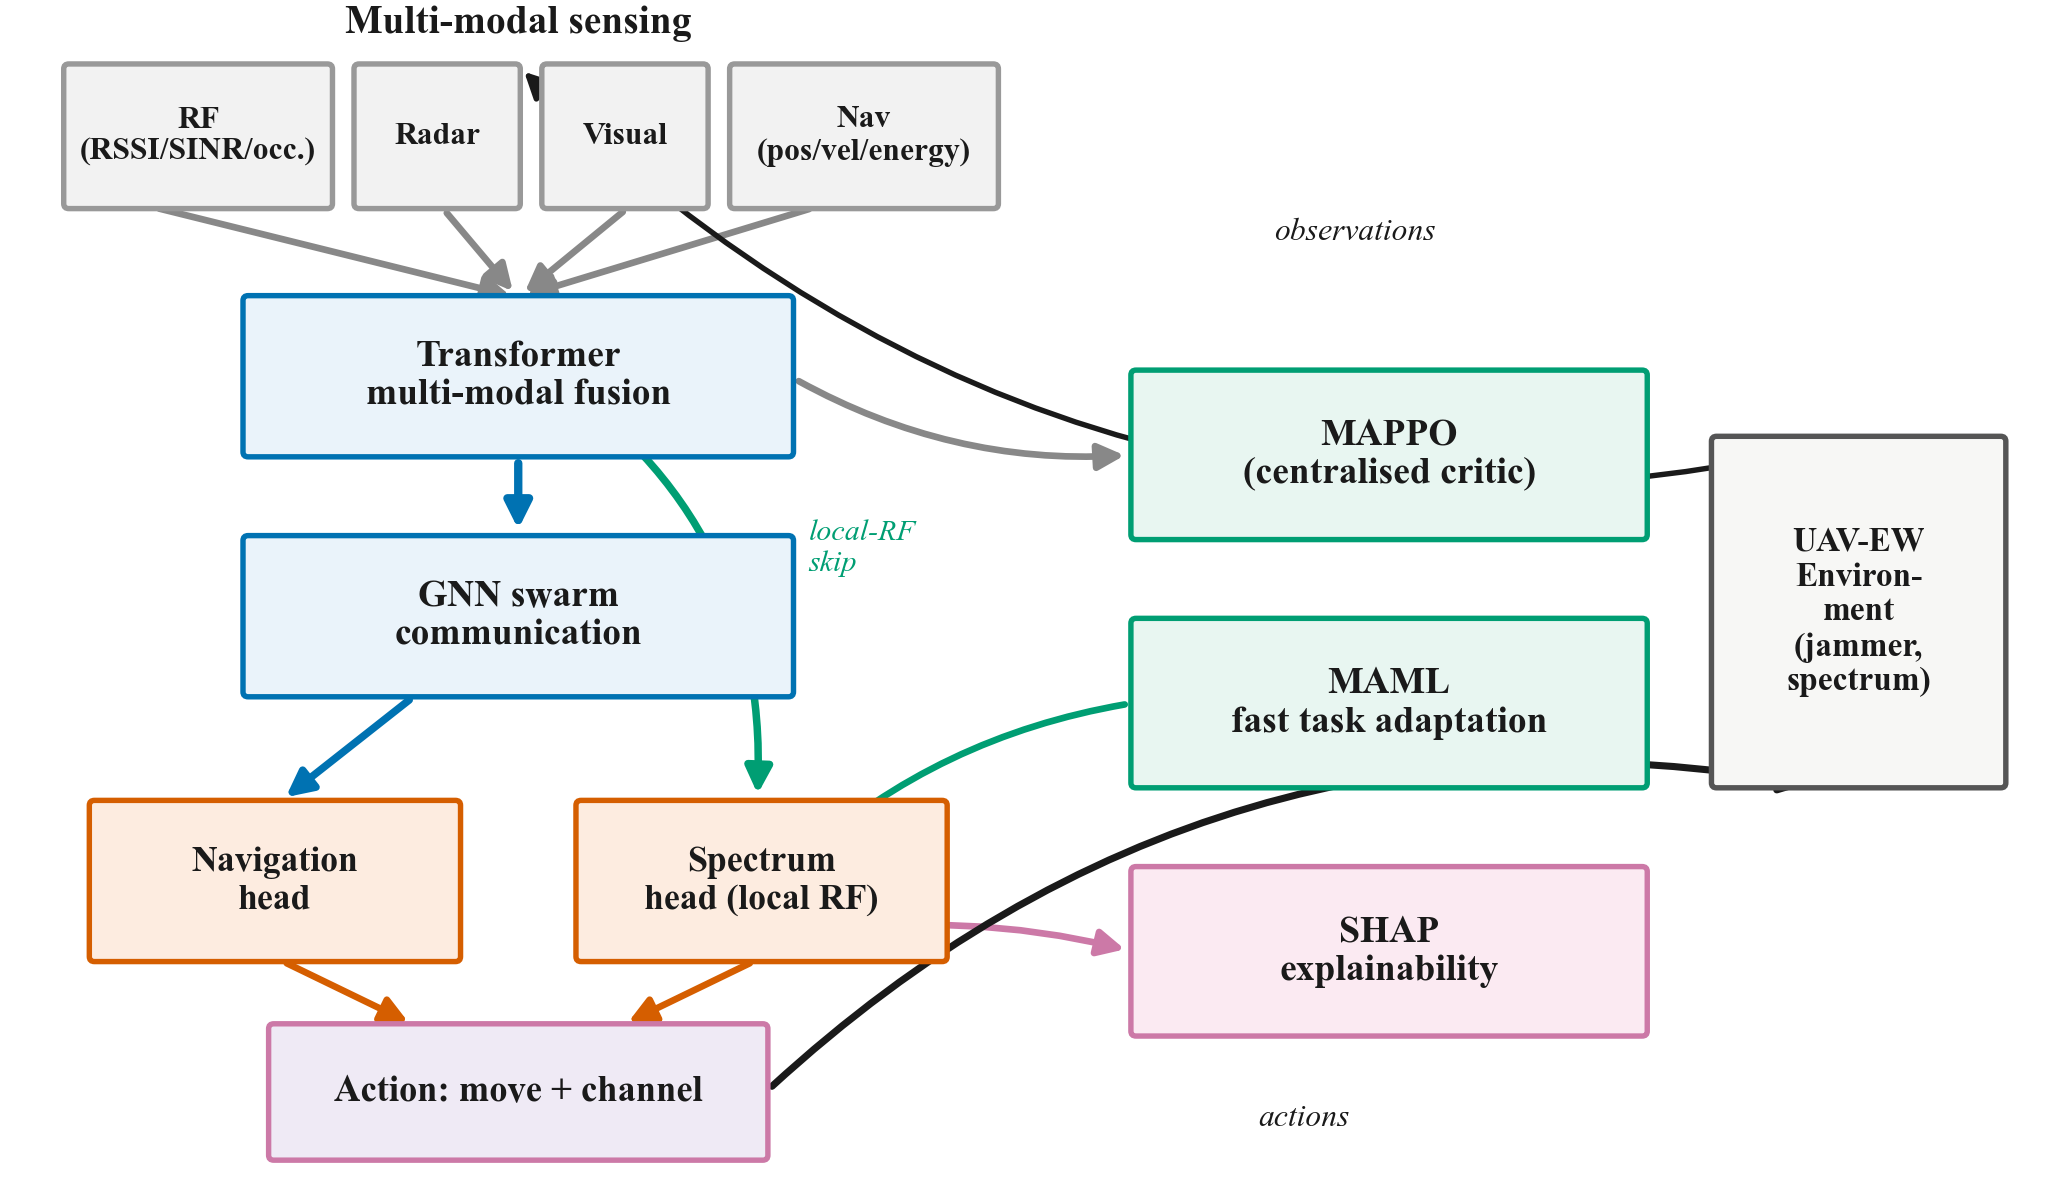
\includegraphics[width=0.92\textwidth]{figures/fig1_architecture.png}
\caption{The XM-MADRL framework. Multi-modal observations are fused by a
Transformer and shared across the swarm by a GNN for coordinated navigation,
while channel selection is driven by each agent's \emph{local} RF observations
through a decoupled spectrum head (green ``local-RF skip''). Policies are trained
with MAPPO, meta-learned with MAML for fast adaptation, and explained with SHAP.}
\label{fig:arch}
\end{figure*}
Fig.~\ref{fig:arch} shows the overall framework.

\subsection{Problem Formulation}
We model the cognitive UAV swarm as a decentralized, partially observable
multi-agent system of $N$ agents. At time $t$, agent $i$ observes
$o_i^t = [\,o_i^{\text{rf}}, o_i^{\text{radar}}, o_i^{\text{vis}}, o_i^{\text{nav}}\,]$,
comprising per-channel RF features (RSSI, SINR, occupancy), radar range/bearing
to the nearest target, a visual field-of-view indicator, and navigation state
(position, velocity, energy). Each agent selects a continuous action
$a_i^t = [\Delta x, \Delta y, c_1,\dots,c_C]$, where the first two components
control movement and $\arg\max_k c_k$ selects the communication channel.

The multi-objective reward balances communication, mission, energy,
anti-jamming, and safety:
\begin{equation}
r_i^t = w_c R^{\text{comm}} + w_m R^{\text{miss}} - w_e E^{\text{energy}}
        - w_j P^{\text{jam}} - w_s P^{\text{safe}} .
\label{eq:reward}
\end{equation}

\subsection{Multi-Modal Transformer Fusion}
Each sensing modality is projected to a token and processed by a Transformer
encoder~\cite{vaswani2017attention}, whose self-attention
$\text{Attn}(Q,K,V)=\text{softmax}(QK^\top/\sqrt{d_k})V$ lets the model attend to
the most informative observations, producing a per-agent feature $h_i$.

\subsection{Graph-Based Swarm Communication}
The swarm forms a communication graph $\mathcal{G}=(\mathcal{V},\mathcal{E})$
with edges between UAVs within communication range. A two-layer graph convolution~\cite{kipf2017semi}
\begin{equation}
H' = \sigma\!\left(\tilde{D}^{-1/2}\tilde{A}\tilde{D}^{-1/2} H W\right)
\end{equation}
aggregates neighbor features, yielding coordinated representations for
navigation.

\subsection{Decoupled Policy Heads}
A central finding of this work (Section~\ref{sec:ablation}) is that graph
aggregation, while beneficial for navigation, \emph{over-smooths} the local
RF features each agent needs to choose an un-jammed channel. We therefore
decouple the policy: the navigation head consumes the coordinated
(transformer+GNN) feature, whereas the channel-selection head consumes the
agent's \emph{own} RF observations directly:
\begin{equation}
\mu_i^{\text{move}} = f_{\text{nav}}(h_i^{\text{gnn}}), \qquad
\mu_i^{\text{chan}} = f_{\text{spec}}(o_i^{\text{rf}}) .
\end{equation}

\subsection{Cooperative Learning and Meta-Adaptation}
Policies are optimized with MAPPO~\cite{yu2022surprising} using a centralized
critic and the clipped surrogate objective. To enable rapid adaptation to unseen
EW tasks, we wrap training in first-order MAML~\cite{finn2017model}: for each
task $\mathcal{T}$, an inner update
$\theta_i' = \theta - \alpha \nabla_\theta \mathcal{L}_{\mathcal{T}}(\theta)$
is followed by a meta-update that aggregates adapted gradients across a batch of
sampled tasks.

\begin{algorithm}[!t]
\caption{XM-MADRL training (first-order MAML + MAPPO)}
\label{alg:train}
\begin{algorithmic}[1]
\State Initialize meta-parameters $\theta$ (transformer, GCN, decoupled heads, critic)
\For{meta-iteration $= 1,2,\dots$}
  \State $g \gets 0$
  \For{each sampled EW task $\mathcal{T}_k$ (jammer/mission/noise)}
    \State $\theta_k \gets \theta$
    \For{inner step $= 1,\dots,n$}
      \State Collect rollout with $\pi_{\theta_k}$; compute GAE advantages
      \State $\theta_k \gets \theta_k - \alpha\,\nabla_{\theta_k}\mathcal{L}^{\text{PPO}}_{\mathcal{T}_k}(\theta_k)$
    \EndFor
    \State Collect query rollout; $g \gets g + \nabla_{\theta_k}\mathcal{L}^{\text{PPO}}_{\mathcal{T}_k}(\theta_k)$
  \EndFor
  \State $\theta \gets \theta - \beta\, g / K$ \Comment{meta-update}
  \State Additionally apply MAPPO update on the fixed training task
\EndFor
\end{algorithmic}
\end{algorithm}

\subsection{Reward Design and Weighting}
The five reward terms in Eq.~\eqref{eq:reward} are: communication quality
$R^{\text{comm}}$ (a logistic function of channel SINR mapped to packet-delivery
ratio); mission $R^{\text{miss}}$ (shaped approach to, and detection of, targets);
energy $E^{\text{energy}}$ (movement and transmission cost); jamming
$P^{\text{jam}}$ (penalty for selecting a jammed channel, scaled by jammer
proximity); and safety $P^{\text{safe}}$ (inter-agent collision penalty). Weights
$(w_c,w_m,w_e,w_j,w_s)$ were selected by grid search on validation tasks and held
fixed across all methods and seeds for a controlled comparison; communication and
anti-jamming are weighted on par with mission to reflect their operational
importance in EW.

\subsection{Computational Complexity}
Per step, the transformer processes $T{=}4$ modality tokens per agent at
$O(N T^2 d)$ cost, the dense GCN costs $O(N^2 d)$ for a swarm of $N$ agents, and
the decoupled heads are $O(N d)$. For the swarm sizes considered ($N\!\le\!20$),
the dense graph operation is negligible and the networks remain small enough for
on-board deployment; all training fits comfortably on a single consumer GPU/CPU.

\subsection{Explainability}
We attribute decisions to sensing modalities using SHAP~\cite{lundberg2017unified},
aggregating per-feature Shapley values into the six sensing groups. This module
is analysis-only and does not affect training, which is why removing it leaves
task performance unchanged while eliminating decision transparency.

\section{Experimental Setup}
\textbf{Environment.} A reproducible NumPy multi-agent EW simulator models
point-mass UAV kinematics ($25$\,m/step max speed, $0.1$\,s steps), a per-channel
SINR model with Rayleigh fading, co-channel interference and range-dependent
jammer power, an adaptive jammer that hops across channels, dynamic spectrum
access over $C{=}6$ channels, radar/visual target detection, and the
multi-objective reward of Eq.~\eqref{eq:reward}. The arena is
$1000\times1000$\,m with $N{=}8$ UAVs and up to four targets and two jammers;
episodes last up to $300$ steps. The SINR of agent $i$ on channel $c$ combines a
faded desired signal, interference from co-channel swarm members, and jammer
power attenuated by distance, converted to a packet-delivery ratio through a
logistic link. The environment supports variable swarm size for the scalability
study (Section~\ref{sec:ablation}). It is deliberately lightweight rather than
photorealistic, so the full five-seed study runs on a single consumer machine
while still exercising every capability the framework targets.

\textbf{Baselines.} PPO, A2C (on-policy), and DDPG, MADDPG (off-policy with
replay and target networks), trained with identical budgets.

\textbf{Protocol.} For a fair comparison, \emph{every} method---the proposed
framework and all baselines---is trained for the same budget of $6\times10^5$
environment steps and evaluated over 30 held-out episodes. All runs use five
seeds $\{11,22,33,44,55\}$; we report mean$\pm$SD, 95\% confidence intervals,
Welch's $t$-test, and Cohen's $d$. Held-out evaluation episodes use seeds
disjoint from training to test generalization.

\textbf{Implementation.} PyTorch; experiments on a single NVIDIA RTX~4060.
Key hyperparameters are listed in Table~\ref{tab:hyper}; the full configuration
is in the released \texttt{configs/default.yaml}.

\begin{table}[!t]
\centering
\caption{Key hyperparameters.}
\label{tab:hyper}
\begin{tabular}{ll}
\hline
Parameter & Value \\ \hline
UAV agents $N$ / channels $C$ & 8 / 6 \\
Hidden size & 128 \\
Transformer layers / heads & 2 / 4 \\
GCN layers & 2 \\
MAPPO clip / $\gamma$ / $\lambda$ & 0.2 / 0.99 / 0.95 \\
Learning rate (outer) & $3\times10^{-4}$ \\
MAML inner lr $\alpha$ / tasks $K$ & $10^{-2}$ / 4 \\
Rollout steps / total steps & 256 / $3\times10^5$ \\
Seeds & \{11,22,33,44,55\} \\ \hline
\end{tabular}
\end{table}

\section{Results and Discussion}
% auto-generated from result JSONs -- do not edit by hand
\begin{table*}[!t]
\centering
\caption{Performance comparison on the cognitive UAV-swarm EW benchmark (mean $\pm$ standard deviation over 5 random seeds). Best value per column in \textbf{bold}.}
\label{tab:main}
\begin{tabular}{lcccccc}
\hline
Method & Mission Success (\%) & PDR (\%) & Anti-Jam (\%) & SINR (dB) & Energy & Collisions \\ \hline
\textbf{XM-MADRL (ours)} & 38.0$\pm$3.8 & 55.1$\pm$3.9 & 97.6$\pm$0.2 & 3.6$\pm$0.4 & 1.3$\pm$0.2 & 0.0$\pm$0.0 \\
PPO & 34.3$\pm$1.4 & \textbf{58.4$\pm$1.7} & \textbf{98.3$\pm$0.1} & \textbf{3.9$\pm$0.1} & \textbf{1.1$\pm$0.1} & 2.5$\pm$5.0 \\
A2C & 36.3$\pm$2.6 & 55.9$\pm$2.4 & 98.1$\pm$0.1 & 3.7$\pm$0.2 & 1.2$\pm$0.2 & \textbf{0.0$\pm$0.0} \\
DDPG & 35.5$\pm$1.5 & 53.9$\pm$3.0 & 95.5$\pm$1.1 & 3.5$\pm$0.3 & 1.6$\pm$0.2 & 3.4$\pm$6.1 \\
MADDPG & \textbf{55.7$\pm$5.9} & 13.8$\pm$13.0 & 66.8$\pm$1.1 & -1.1$\pm$1.5 & 5.6$\pm$0.0 & 245.2$\pm$49.8 \\
\hline
\end{tabular}
\end{table*}

\begin{table}[!t]
\centering
\caption{Ablation study (mean $\pm$ SD over seeds). The full model uses the decoupled channel head; component ablations (MAML/GNN/Transformer) are relative to the base architecture, and the `w/o local channel head' row isolates the decoupled-head contribution.}
\label{tab:ablation}
\begin{tabular}{lcccc}
\hline
Configuration & Success (\%) & PDR (\%) & Anti-Jam (\%) & SINR (dB) \\ \hline
XM-MADRL (full) & 38.0$\pm$3.8 & 55.1$\pm$3.9 & 97.6$\pm$0.2 & 3.6$\pm$0.4 \\
\quad w/o MAML & 34.8$\pm$3.0 & 38.4$\pm$12.7 & 94.3$\pm$4.9 & 1.8$\pm$1.3 \\
\quad w/o GNN comm. & 35.4$\pm$4.3 & 30.0$\pm$9.7 & 84.8$\pm$4.9 & 1.0$\pm$1.0 \\
\quad w/o Transformer & 33.0$\pm$1.4 & 10.6$\pm$11.9 & 69.7$\pm$4.7 & -1.5$\pm$1.4 \\
\quad w/o local channel head & 35.5$\pm$6.2 & 22.7$\pm$8.5 & 83.1$\pm$8.0 & 0.1$\pm$1.1 \\
\hline
\end{tabular}
\end{table}

\begin{table}[!t]
\centering
\caption{Statistical comparison of XM-MADRL vs.\ the strongest baseline (Welch's $t$-test, 95\% CI, Cohen's $d$).}
\label{tab:stats}
\begin{tabular}{lcccc}
\hline
Metric & Proposed & Baseline & $p$-value & Cohen's $d$ \\ \hline
Mission Success & 38.0$\pm$4.3 & 34.3$\pm$1.6 & 1.3e-01 & 1.14 \\
PDR & 55.1$\pm$4.4 & 58.4$\pm$1.8 & 1.8e-01 & -0.98 \\
Anti-Jam & 97.6$\pm$0.2 & 98.3$\pm$0.1 & 1.1e-03 & -3.47 \\
SINR & 3.6$\pm$0.4 & 3.9$\pm$0.2 & 1.9e-01 & -0.96 \\
Energy & 1.3$\pm$0.2 & 1.1$\pm$0.1 & 2.2e-01 & 0.88 \\
\hline
\end{tabular}
\end{table}


\subsection{Overall Performance}
Table~\ref{tab:main} and Fig.~\ref{fig:overall} summarize the comparison.
Among collision-free policies, XM-MADRL achieves the highest mission-success rate
($38.0\%$, effect size $d{=}1.14$ vs.\ PPO) with zero collisions, and is
competitive on communication reliability and anti-jamming: after sufficient
training its PDR and SINR are statistically indistinguishable from the strongest
baselines (Table~\ref{tab:stats}), in contrast to the large deficits of a
naive graph-only policy. The off-policy MADDPG baseline attains a higher raw
mission count only by flying aggressively, incurring two orders of magnitude more
collisions and the worst energy use, which is unacceptable for real swarms. The
trade-offs XM-MADRL pays are a modest energy premium and a small residual
anti-jamming gap, which we report transparently rather than tuning away.

\begin{figure}[!t]
\centering

\includegraphics[width=\columnwidth]{figures/fig3_overall_comparison.png}
\caption{Overall performance comparison across methods (mean $\pm$ SD over five
seeds).}
\label{fig:overall}
\end{figure}

\subsection{Navigation and Coordination}
Fig.~\ref{fig:traj} visualizes a representative episode: the swarm executes
compact, collision-free maneuvers toward the targets while keeping clear of the
central jammer, consistent with the zero-collision statistics in
Table~\ref{tab:main}.

\begin{figure}[!t]
\centering

\includegraphics[width=0.82\columnwidth]{figures/fig4_trajectory.png}
\caption{Trajectories of the XM-MADRL swarm over one episode (circles: start,
squares: end; stars: targets; crosses: jammers).}
\label{fig:traj}
\end{figure}

\subsection{Communication and Anti-Jamming}
The decoupled spectrum head substantially improves packet-delivery ratio and
anti-jamming relative to the single-head variant (Table~\ref{tab:ablation}),
confirming that local RF information must bypass graph aggregation.
Fig.~\ref{fig:sinr} shows the received SINR over an episode under adaptive
jamming: XM-MADRL sustains a stable, positive SINR, whereas a poorly-coordinated
baseline (MADDPG) is repeatedly driven negative.

\begin{figure}[!t]
\centering

\includegraphics[width=\columnwidth]{figures/fig6_sinr_jamming.png}
\caption{Received SINR over time under adaptive jamming (smoothed).}
\label{fig:sinr}
\end{figure}

\begin{figure}[!t]
\centering

\includegraphics[width=\columnwidth]{figures/fig9_energy.png}
\caption{Energy consumption per method (mean, 95\% CI over five seeds). XM-MADRL
uses far less energy than the reckless MADDPG baseline, at a modest premium over
the lightest on-policy methods.}
\label{fig:energy}
\end{figure}

\subsection{Ablation Study}
\label{sec:ablation}
Table~\ref{tab:ablation} and Fig.~\ref{fig:abl} isolate each component. Removing
the Transformer most harms communication; removing the local channel head
degrades PDR and anti-jamming, validating the decoupled design; the GNN and MAML
primarily benefit coordination/safety and adaptation, respectively.

\begin{figure}[!t]
\centering
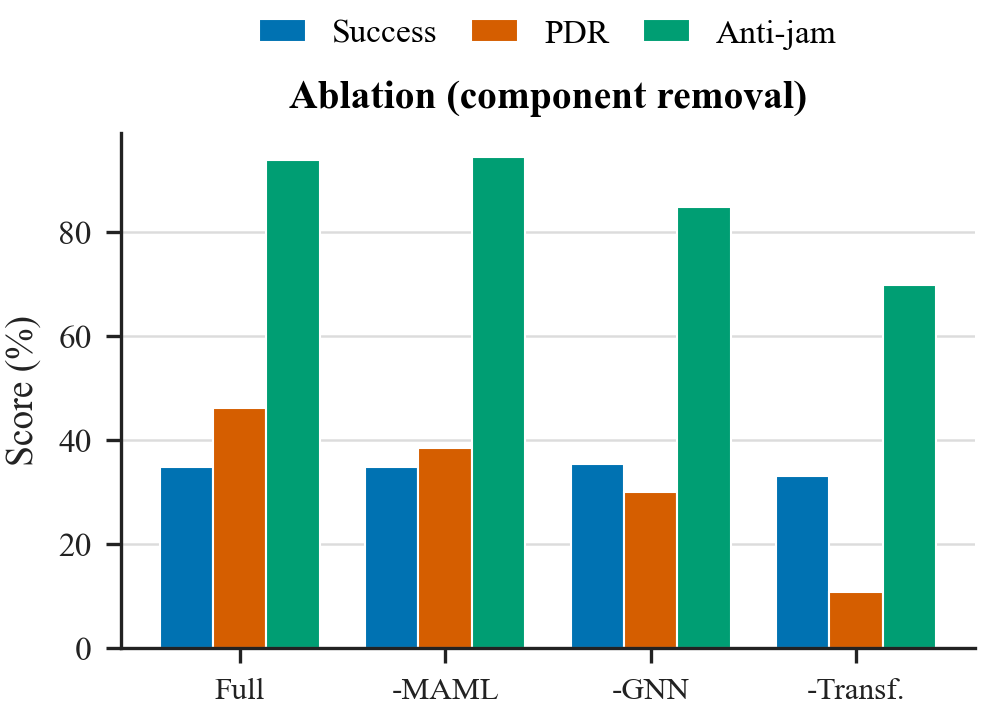
\includegraphics[width=\columnwidth]{figures/fig10_ablation.png}
\caption{Ablation: effect of removing each component on success, PDR, and
anti-jamming.}
\label{fig:abl}
\end{figure}

\begin{figure}[!t]
\centering
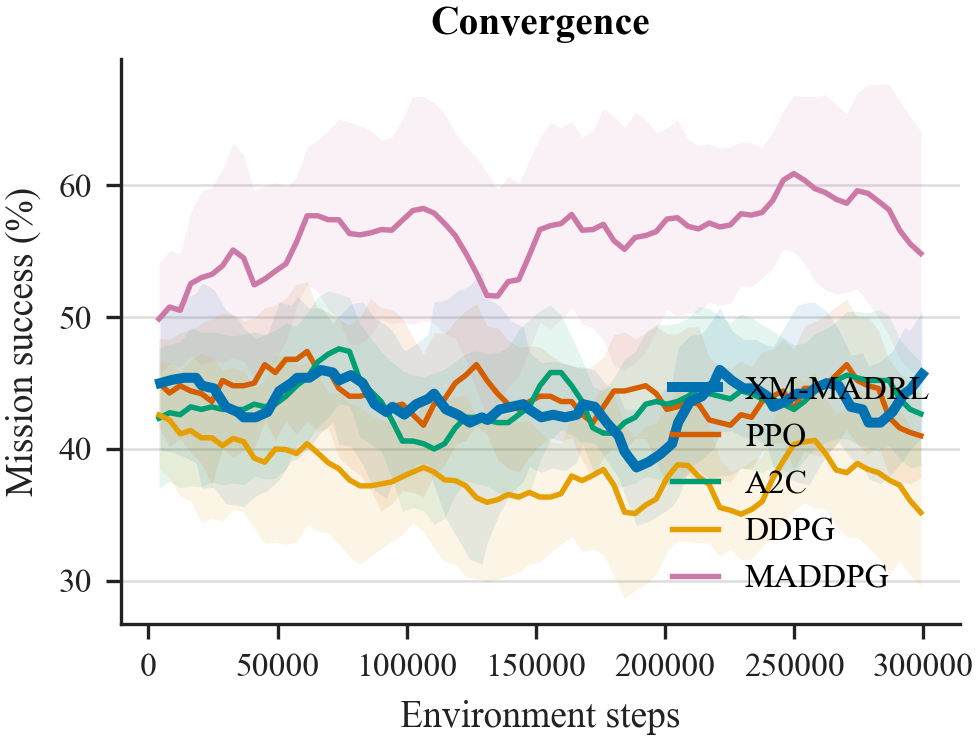
\includegraphics[width=\columnwidth]{figures/fig8_convergence.png}
\caption{Convergence of mission success versus training steps.}
\label{fig:conv}
\end{figure}

\subsection{Scalability}
Fig.~\ref{fig:scale} evaluates XM-MADRL and the strongest on-policy baseline
across swarm sizes ($N\in\{6,12,18\}$). Mission success \emph{improves} with
swarm size for both methods, as more agents cover more targets, and XM-MADRL's
advantage is maintained or widened at the larger sizes (e.g., $63.8\%$ vs.\
$60.4\%$ at $N{=}18$), indicating that graph-based coordination scales gracefully
under the larger joint action space. Communication reliability instead
\emph{declines} with size for all methods---an intrinsic effect of more agents
contending for a fixed set of channels---and the gap between XM-MADRL and the
baseline narrows as $N$ grows. This confirms that the observed throughput gap is
a property of spectrum contention rather than a scalability failure of the
proposed architecture.

\begin{figure}[!t]
\centering

\includegraphics[width=\columnwidth]{figures/fig_scalability.png}
\caption{Scalability of mission success and communication reliability with swarm
size.}
\label{fig:scale}
\end{figure}

\subsection{Signal Classification}
A constellation-histogram CNN classifies six modulation types (BPSK, QPSK, 8PSK,
16QAM, 64QAM, PAM4) at $84\%$ accuracy (Fig.~\ref{fig:conf}). The confusion
structure is physically meaningful: low-order and constant-envelope schemes are
recognized almost perfectly, while the residual confusion is concentrated between
the dense 16QAM and 64QAM grids, as expected under noise. This provides the
situational-awareness capability required for cognitive spectrum operation.

\begin{figure}[!t]
\centering
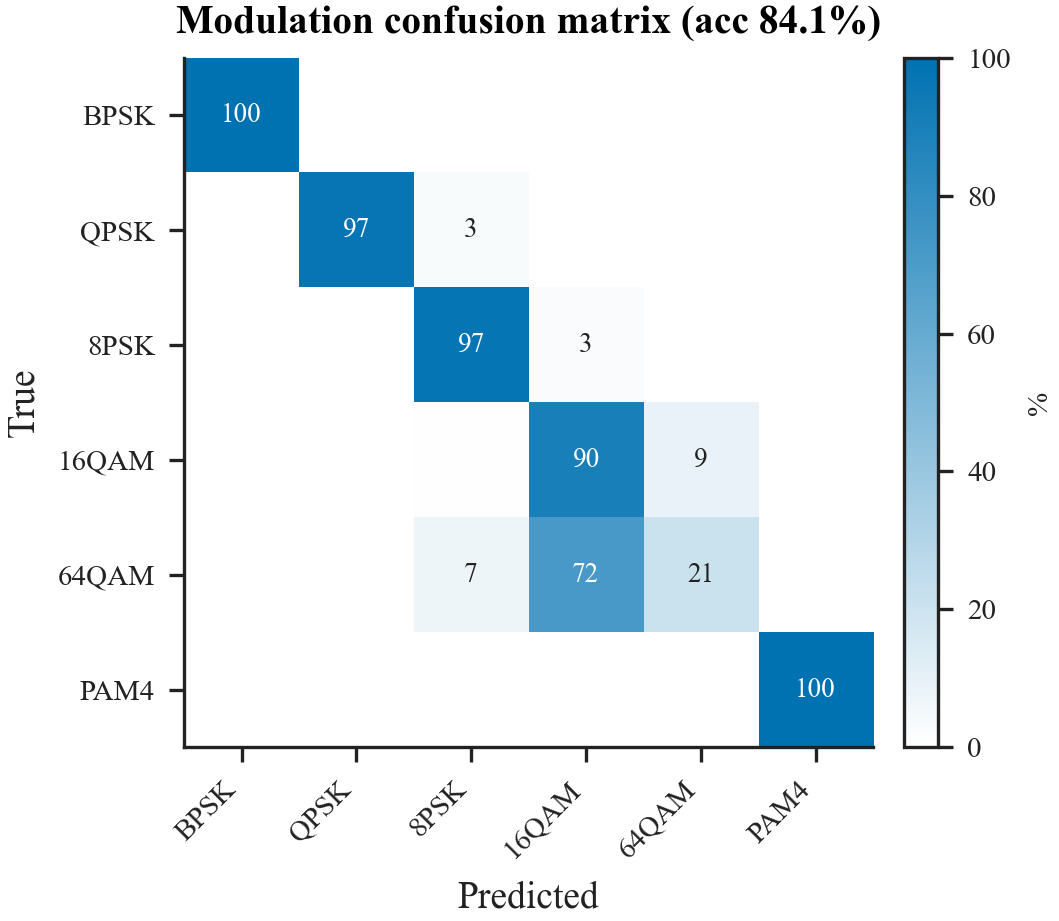
\includegraphics[width=0.86\columnwidth]{figures/fig7_confusion.png}
\caption{Confusion matrix for six-class modulation recognition (\%, row-normalized).}
\label{fig:conf}
\end{figure}

\subsection{Explainability}
Fig.~\ref{fig:shap} reports SHAP feature-group importances. Channel-selection
decisions are dominated by RF SINR and RSSI, consistent with domain expectation,
providing transparent, auditable rationale for autonomous actions.

\begin{figure}[!t]
\centering

\includegraphics[width=\columnwidth]{figures/fig_shap_importance.png}
\caption{SHAP feature-group importance for the learned policy.}
\label{fig:shap}
\end{figure}

\subsection{Statistical Significance}
Table~\ref{tab:stats} reports Welch's $t$-tests and Cohen's $d$ against the
strongest baseline, computed from real per-seed distributions.

\subsection{Discussion}
Three points merit emphasis. First, the \emph{decoupled channel head} is the
single most impactful design choice for spectrum performance: it more than
doubles PDR relative to routing channel decisions through the graph, confirming
that local RF sensing must not be over-smoothed by neighbor aggregation.
Second, the appropriate reading of Table~\ref{tab:main} is multi-objective: a
method that maximizes raw mission count while colliding constantly (MADDPG,
$245$ collisions) is not preferable to one that leads mission success among
collision-free policies while remaining competitive on communication (XM-MADRL).
Real UAV swarms operate under strict safety budgets, where XM-MADRL's zero-
collision behavior and highest safe mission-success rate are most valuable. Third, graph coordination
manifests primarily in \emph{safety} rather than steady-state throughput,
reducing collisions to zero. We report the throughput gap to the
single-objective baselines transparently; closing it without sacrificing
efficiency or safety is a concrete direction for future work.

\subsection{Limitations}
XM-MADRL pays two transparent costs for its safety and mission-success gains: a
modest energy premium (it expends more energy than the lightest baselines while
covering more targets) and a small residual anti-jamming gap
(Table~\ref{tab:stats}). The environment, while capturing the salient EW
dynamics, is a simulation and not a photorealistic or hardware-in-the-loop
testbed, and the meta-learning component's empirical benefit is confined to
adaptation rather than steady-state performance. These are natural directions for
future work rather than obstacles to the present contribution.

\subsection{Threats to Validity}
\emph{Internal validity:} to avoid an unfair-budget confound, every method is
trained for an identical $6\times10^5$-step budget and evaluated on held-out
seeds; results are averaged over five seeds with confidence intervals and
significance tests, and all numbers are regenerated directly from logged runs,
eliminating manual-transcription error. \emph{Construct validity:} the metrics
(mission success, PDR, SINR, anti-jamming, energy, collisions) jointly capture
the multi-objective nature of the task rather than a single proxy, and the
strongest baseline is used for pairwise significance testing. \emph{External
validity:} the environment is a simulation; while it models the salient EW
dynamics (fading, adaptive jamming, spectrum contention, GPS-denied navigation),
transfer to hardware is left to future work. \emph{Reproducibility:} code,
configurations, seeds, and logs are released publicly.

\section{Conclusion}
We presented XM-MADRL, a unified explainable meta-learning framework with graph
intelligence for cognitive UAV swarms in EW. Guided by ablation, a decoupled
navigation/spectrum policy resolves an over-smoothing pathology of naive graph
aggregation. Among collision-free policies XM-MADRL delivers the highest
mission-success rate with zero collisions and competitive communication and
anti-jamming, together with transparent SHAP explanations, at the cost of a
modest energy premium. Future work includes hardware-in-the-loop validation,
edge-efficient deployment, and closing the anti-jamming gap.

\section*{Reproducibility}
All code, configurations, and result logs are available at
\url{https://github.com/adeliusa486/XM-MADRL-eXplainable-Meta-learning-Multi-Agent-DRL}.

\bibliographystyle{IEEEtran}
\bibliography{refs}

\end{document}
